\documentclass{article}

\usepackage[a4paper, bottom=0.5in, top=0.5in, left=0.5in, right=0.5in]{geometry}
\usepackage{wrapfig}
\usepackage{natbib}
\usepackage{url}
\usepackage{xcolor}
\usepackage{caption}
\usepackage{hyperref}
\hypersetup{
    colorlinks=true,    
    urlcolor=cyan,
}
\usepackage{bytefield}

\usepackage{amsfonts}
\usepackage{float}
\usepackage{enumitem}

\usepackage{minted}

\usepackage{xparse} % NewDocumentCommand, IfValueTF, IFBooleanTF
\usepackage{tikz-timing}[2014/10/29]
\NewDocumentCommand{\busref}{som}{\texttt{%
		#3%
		\IfValueTF{#2}{[#2]}{}%
		\IfBooleanTF{#1}{\#}{}%
}}


\newcommand{\bitFormat}[1]{\emph{\textbf{\textcolor{cyan}{#1}}}}

\newcommand{\regFormat}[1]{\textbf{\textcolor{magenta}{#1}}}

\newcommand{\pinFormat}[1]{\emph{\textcolor{red}{#1}}}


\usepackage{graphicx}
\graphicspath{ {./Resources/pics/} }



\title{ATmega328P Timer/Counter 1}
\author{Narendiran S}
\date{\today}

\begin{document}
\maketitle

\section{Features}
\begin{itemize}
    \item General purpose 16-bit PWM/Counter module.
    \item Two independent output compare units and One input capture unit
    \item Variable PWM.
    \item Four independent interrupt sources (TOV0, OCF0A, OCF1B and ICF1).
    \item Clear timer on compare match (auto reload)
\end{itemize}

\section{Block Diagram}
\begin{figure}[H]
    \begin{center}
        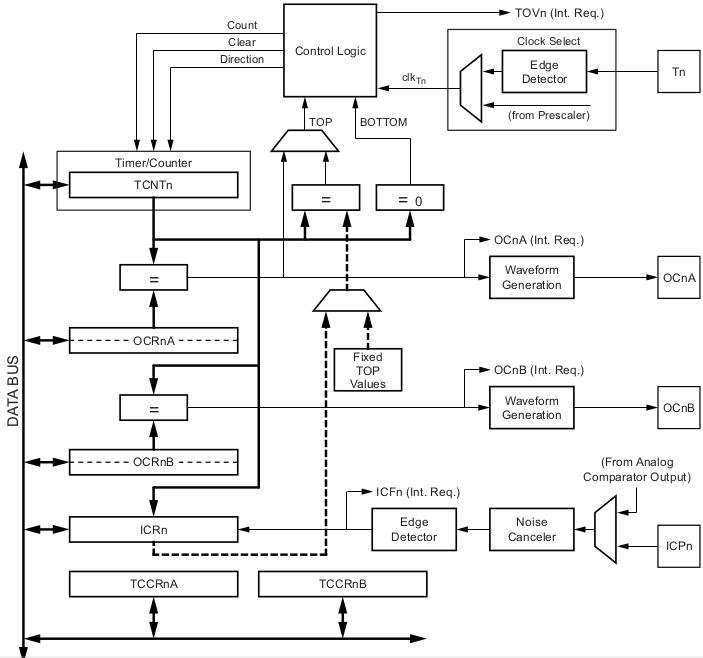
\includegraphics[height=0.6\textheight]{Timer1BlockDiagram.png}
    \end{center}
\end{figure}

\section{Terminologies and Registers}
\begin{minipage}{0.4\textwidth}
    \begin{tabular}{c|p{4.5cm}}
        \textbf{Parameter} & \textbf{Description}\\
        \hline
        BOTTOM & counter reaches 0x0000\\
        MAX & ounter reaches 0xFFFF\\
        TOP & counter reaches highest value (depends on mode of operation can be 0xFF, 0x1FF, 0x3FF, OCR1A, ICR1)
    \end{tabular}
\end{minipage}
\begin{minipage}{0.55\textwidth}
    \begin{tabular}{c|p{5.5cm}}
        \textbf{Register - 16 bit} & \textbf{Name}\\
        \hline
        \regFormat{TCN10} & Timer/Counter1count value\\
        \regFormat{TCCR1A} & Timer/Coutner1 Control Register A\\
        \regFormat{TCCR1B} & Timer/Coutner1 Control Register B\\
        \regFormat{OCBR1A} & Output compare register A\\
        \regFormat{OCBR1B} & Output compare register B\\
        \regFormat{TIFR1} & Timer Interrupt Flag Register\\
        \regFormat{TIMSK1} & Timer interrupt Mask Register\\
        \regFormat{ICR1} & Input Capture Register\\
    \end{tabular}
\end{minipage}

\section{Timer/Counter0 Units}


\end{document}